\section{Matériel et méthodes}
\subsection{Modèle animal}
\lipsum[1]
\subsection{Traitement expérimental}
\subsubsection{Hypergravité}
\label{hypergravite} % on peut mettre systématiquement un \label après chaque titre de partie au cas où un /ref{} serait nécessaire
L'hypergravité consiste à augmenter la force du vecteur gravitaire en lui sur-imposant la force centrifuge. En effet, la force centrifuge induite par la rotation se surimpose à la gravité terrestre ce qui permet d'avoir une force résultante dépendante de la vitesse de rotation. On utilise pour cela des centrifugeuses qui sont des carrousels équipés de nacelles suspendues à des axes libres permettant à la force résultante d'être perpendiculaire au plancher de la nacelle et ainsi obtenir une \og gravité \fg{} dont la force est supérieure à la gravité terrestre tout en maintenant, pour les individus expérimentaux, l'orientation \og naturelle \fg{} de celle-ci.
\lipsum[1-5]
\subsubsection{La centrifugeuse}
Les caractéristiques techniques de la \index{centrifugeuse} ont été décrites dans un article de \cite{jamon_ground-based_2008} et dans la partie \ref{hypergravite}. Brièvement, la centrifugeuse (Figure~\ref{photo_centrifugeuse}) est de grand diamètre (jusqu'à 3,6~m en rotation). Pour limiter les vibrations, la centrifugeuse repose sur des dispositifs anti-vibrations. Le bruit produit par la centrifugeuse est faible. A un mètre de distance, le niveau sonore n'est que de 58~dB contre 52~dB si la centrifugeuse est arrêtée. Les nacelles sont sur des axes libres et chacune peut contenir trois cages de type standard (364x206x131 mm) avec 4 souris par cage, soit un total de 48 souris. La centrifugeuse est équipée de caméras infra-rouge couplées à un système de vidéo-surveillance accessible sur internet. Cela nous permet de contrôler les niveaux d'eau et de nourriture ainsi que de conduire des études de l'activité des individus expérimentaux à distance, de jour comme de nuit. La quantité d'eau et de nourriture disponible par cage permet de faire fonctionner la centrifugeuse 3 semaines sans interruption. Les animaux ont à disposition 400~g de nourriture et 500~ml d'eau, mais la consommation de nourriture sur cette période est en moyenne de 209~g ($\pm$14), et la consommation d'eau de 258 ml ($\pm$21) pour une cage de 4 souris. 
\begin{figure}[h!tbp] % à voir
\vspace{0.5cm}
\setcapindent{2em}
  \centering
  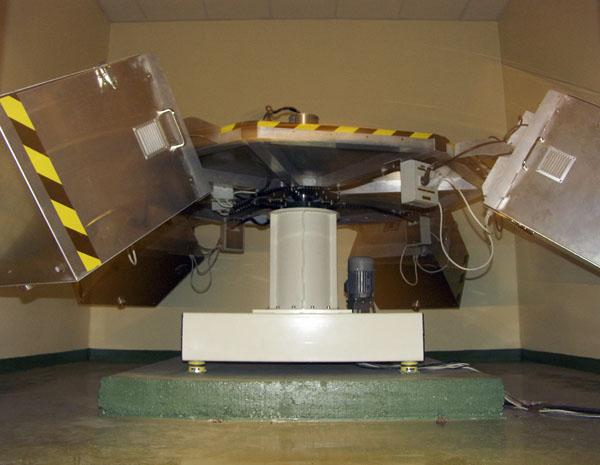
\includegraphics[width=0.7\textwidth]{photo_centrifugeuse}
  \caption[Photographie de la centrifugeuse]{Photographie de la centrifugeuse utilisée.}
  \label{photo_centrifugeuse}
\end{figure}
\lipsum[1]
\section{Deuxième section de la deuxième partie}
\lipsum[2]
\subsection{Première sous-section de la deuxième section de la deuxième partie}
\lipsum[4]
\subsection[Sous-sous-sous-partie]{Deuxième sous-section de la deuxième section de la deuxième partie} % entre [] pour affichage dans la TOC
\lipsum[4]
\subsubsection{Ce titre de section ne s'affiche pas dans la TOC : tocdepth=2}
Nam dui ligula, fringilla a, euismod sodales, sollicitudin vel, wisi \parencite{zohdy_mapping_2012}. \lipsum[3] % citation entre parenthèses et tous les auteurs
\paragraph{Ce titre de section n'est pas numéroté : secnumdepth=3}~~\\ % "~~\\" fait le saut de ligne après le titre de 'paragraph'

% ce saut de ligne dans le code indente 'paragraph'
\lipsum[3]